\chapter{Implementasi dan Pengujian}
\label{chap:implementasi dan pengujian}

\section{Lingkungan Implementasi}
\label{sec:lingkungan implementasi}

Pada subab ini akan dipaparkan perangkat keras dan perangkat lunak yang digunakan dalam membangun sistem rekomendasi program studi Universitas Katolik Parahyangan.

\subsection{Lingkungan Perangkat Keras}
\label{sec:perangkat keras}

\begin{enumerate}
    \item Processor : Intel Core i5-7200
    
    \item Memory : 12 GB
    
    \item Harddisk : 1 T
    
    \item VGA : NVIDIA GeForce 940MX
\end{enumerate}

\section{Lingkungan Perangkat Lunak}
\label{sec:perangkat lunak}

\begin{enumerate}
    \item Web Server : Apache 2.4.41
    
    \item Tools : XAMPP 3.2.4 dan Visual Studio Code
    
    \item Bahasa Pemrograman : PHP 7.4.1
    
    \item Database management system : MySQL
    
    \item Operating System : Windows 10
\end{enumerate}

\section{Implementasi Tabel Basis Data}
\label{sec:implementasi tabel basis data}

Dibawah ini merupakan implementasi tabel basis data yang digunakan pada sistem rekomendasi program studi Universitas Katolik Parahyangan. 

\lstset{numbers=left}

\begin{enumerate}
    \item Tabel Jurusan SMA\\
    Tabel jurusan SMA digunakan untuk menyimpan seluruh data jurusan SMA yang digunakan pada sistem rekomendasi.
    
    \begin{lstlisting}[language=SQL, caption=Implementasi tabel jurusan SMA]
CREATE TABLE `jurusan_sma` ( 
    `id_jurusan` int(10) UNSIGNED NOT NULL,
    `nama_jurusan` varchar(25) COLLATE utf8mb4_unicode_ci NOT NULL
) ENGINE=InnoDB DEFAULT CHARSET=utf8mb4 COLLATE=utf8mb4_unicode_ci;
    \end{lstlisting}
    
    \item Tabel Fakultas\\
    Tabel fakultas digunakan untuk menyimpan seluruh fakultas yang ada di Universitas Katolik Parahyangan.
    
    \begin{lstlisting}[language=SQL, caption=Implementasi tabel ]
CREATE TABLE `fakultas` (
    `id_fakultas` int(10) UNSIGNED NOT NULL,
    `nama_fakultas` varchar(50) COLLATE utf8mb4_unicode_ci NOT NULL
) ENGINE=InnoDB DEFAULT CHARSET=utf8mb4 COLLATE=utf8mb4_unicode_ci;    
    \end{lstlisting}

    \item Program Studi\\
    Tabel program studi digunakan untuk menyimpan seluruh program studi yang ada di Universitas Katolik Parahyangan.
    
    \begin{lstlisting}[language=SQL, caption=Implementasi tabel ]
CREATE TABLE `program_studi` (
    `id_program_studi` int(10) UNSIGNED NOT NULL,
    `nama_program_studi` varchar(50) COLLATE utf8mb4_unicode_ci NOT NULL,
    `id_fakultas` int(10) UNSIGNED NOT NULL,
    `id_jurusan` int(10) UNSIGNED NOT NULL
) ENGINE=InnoDB DEFAULT CHARSET=utf8mb4 COLLATE=utf8mb4_unicode_ci;
    
    \end{lstlisting}
    
    \item Mahasiswa\\
    Tabel mahasiswa digunakan untuk menyimpan nilai seluruh mahasiswa yang sudah lulus dari Universitas Katolik Parahyangan.
    
    \begin{lstlisting}[language=SQL, caption=Implementasi tabel ]
CREATE TABLE `mahasiswa` (
    `id_mahasiswa` int(10) UNSIGNED NOT NULL,
    `NPM` varchar(10) COLLATE utf8mb4_unicode_ci NOT NULL,
    `IPK` double(3,2) NOT NULL,
    `id_jurusan` int(10) UNSIGNED NOT NULL,
    `id_program_studi` int(10) UNSIGNED NOT NULL
) ENGINE=InnoDB DEFAULT CHARSET=utf8mb4 COLLATE=utf8mb4_unicode_ci;    
    \end{lstlisting}
    
    \item Mata Pelajaran\\
    Tabel mata pelajaran digunakan untuk menyimpan mata pelajaran yang digunakan pada PMDK di Universitas Katolik Parahyangan.
    
    \begin{lstlisting}[language=SQL, caption=Implementasi tabel ]
CREATE TABLE `mata_pelajaran` (
    `id_mata_pelajaran` int(10) UNSIGNED NOT NULL,
    `nama_mata_pelajaran` varchar(20) COLLATE utf8mb4_unicode_ci NOT NULL
) ENGINE=InnoDB DEFAULT CHARSET=utf8mb4 COLLATE=utf8mb4_unicode_ci;

    \end{lstlisting}
    
    \item Nilai\\
    Tabel nilai digunakan untuk menyimpan nilai mahasiswa pada kelas X dan XI untuk semester 1 dan 2 pada saat SMA.
    
    \begin{lstlisting}[language=SQL, caption=Implementasi tabel ]
CREATE TABLE `nilai` (
    `id_nilai` int(10) UNSIGNED NOT NULL,
    `id_mata_pelajaran` int(10) UNSIGNED NOT NULL,
    `id_mahasiswa` int(10) UNSIGNED NOT NULL,
    `101` double(5,2) NOT NULL,
    `102` double(5,2) NOT NULL,
    `111` double(5,2) NOT NULL,
    `112` double(5,2) NOT NULL,
    `AVG` double(5,2) NOT NULL
) ENGINE=InnoDB DEFAULT CHARSET=utf8mb4 COLLATE=utf8mb4_unicode_ci;
    \end{lstlisting}
    
\end{enumerate}

\section{Impelemtasi Antar Muka}
\label{sec:implementasi antar muka}

Pada subab ini akan ditampilkan antar muka yang digunakan pada sistem rekomendasi program studi Universitas Katolik Parahyangan.

\begin{enumerate}
    \item Halaman index saat siswa/i mengakses sistem
    
    \begin{figure}[H]
        \centering
        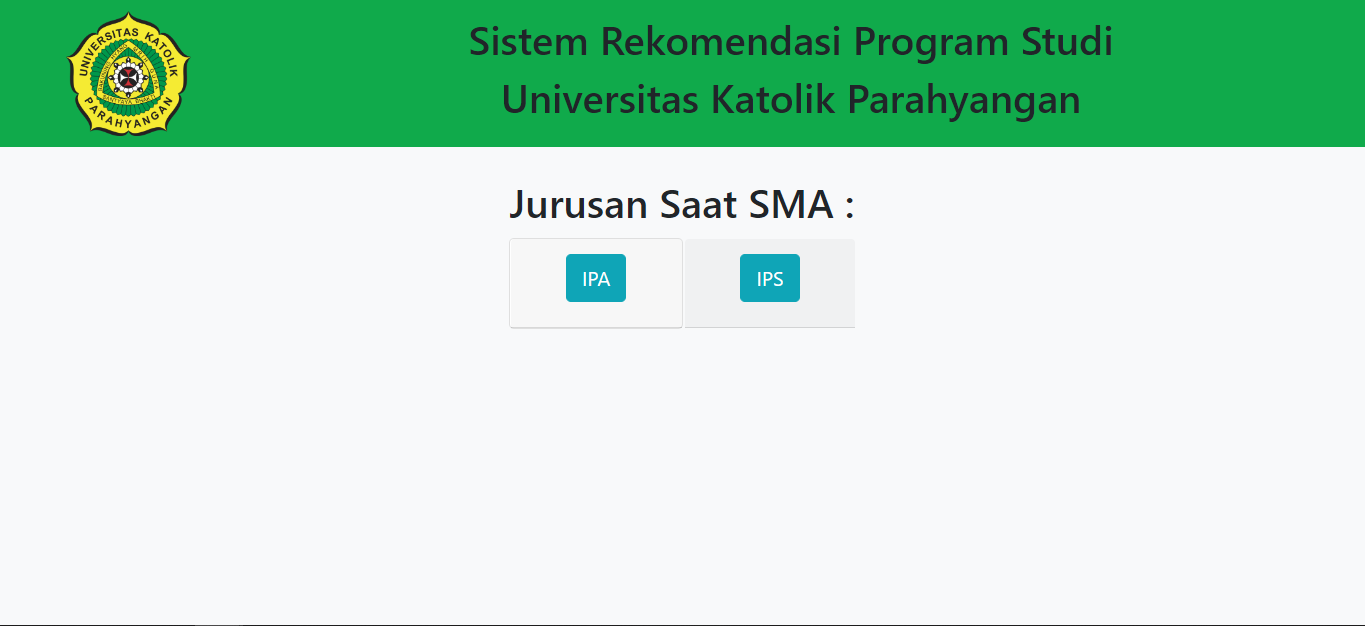
\includegraphics[width = 12cm, height =8 cm]{doc/DokumenSkripsi/Gambar/gambar51.png}
        \caption{Halaman Index Sistem}
        \label{fig:gambar51}
    \end{figure}
    
    \item Halaman pengisisian nilai siswa/i IPA
    
    \begin{figure}[H]
        \centering
        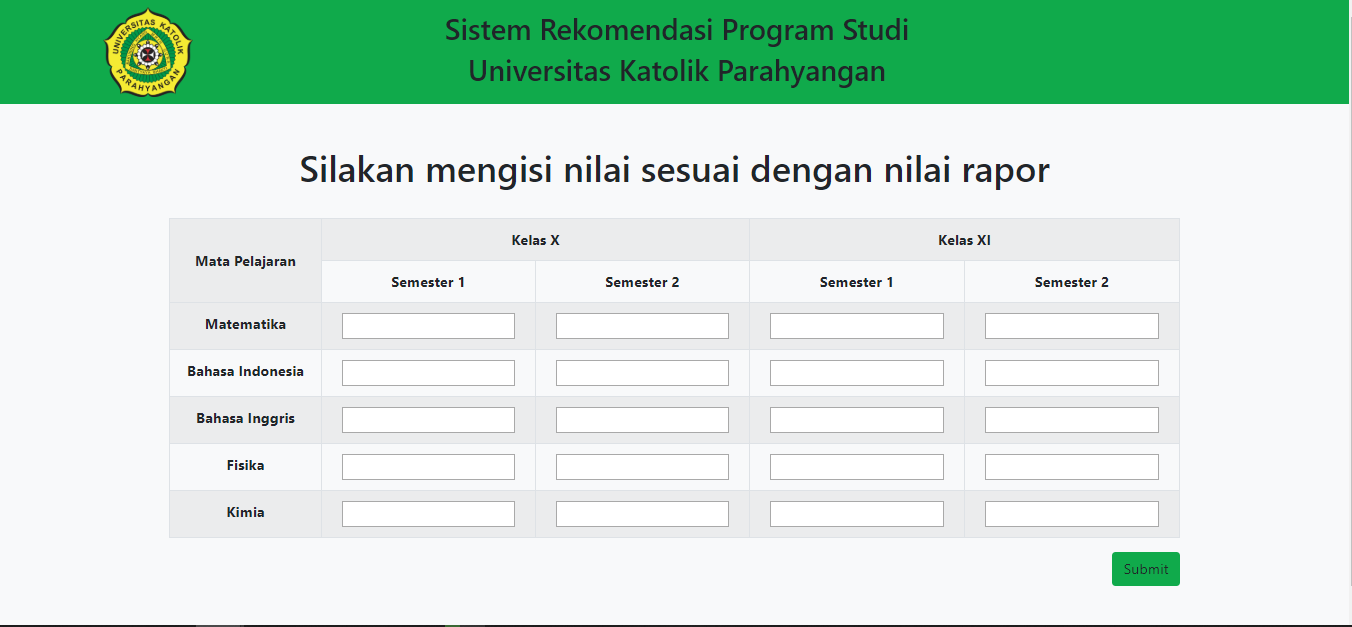
\includegraphics[width = 12cm, height =8 cm]{doc/DokumenSkripsi/Gambar/gambar52.png}
        \caption{Halaman Index Pengisian Nilai IPA}
        \label{fig:gambar52}
    \end{figure}
    
    \item Halaman pengisisian nilai siswa/i IPS
    
    \begin{figure}[H]
        \centering
        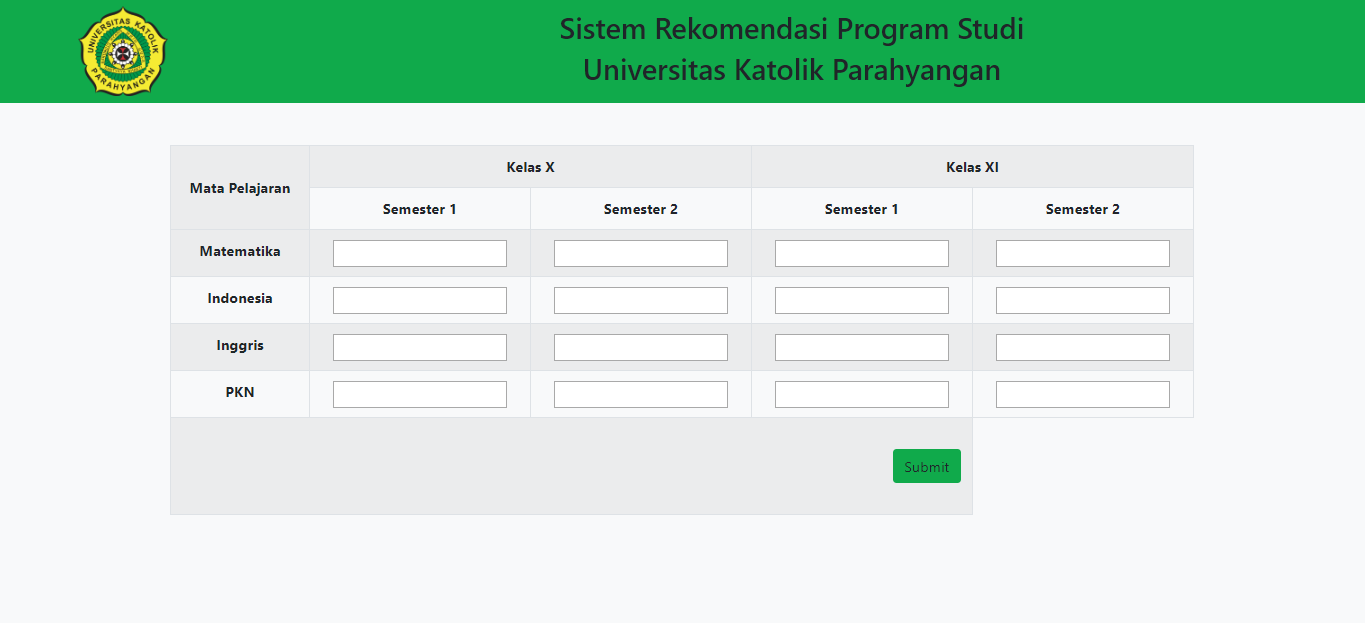
\includegraphics[width = 12cm, height =8 cm]{doc/DokumenSkripsi/Gambar/gambar53.png}
        \caption{Halaman Index Pengisian Nilai IPS}
        \label{fig:gambar53}
    \end{figure}
    
    \item Halaman hasil rekomendasi
    \begin{figure}[H]
        \centering
        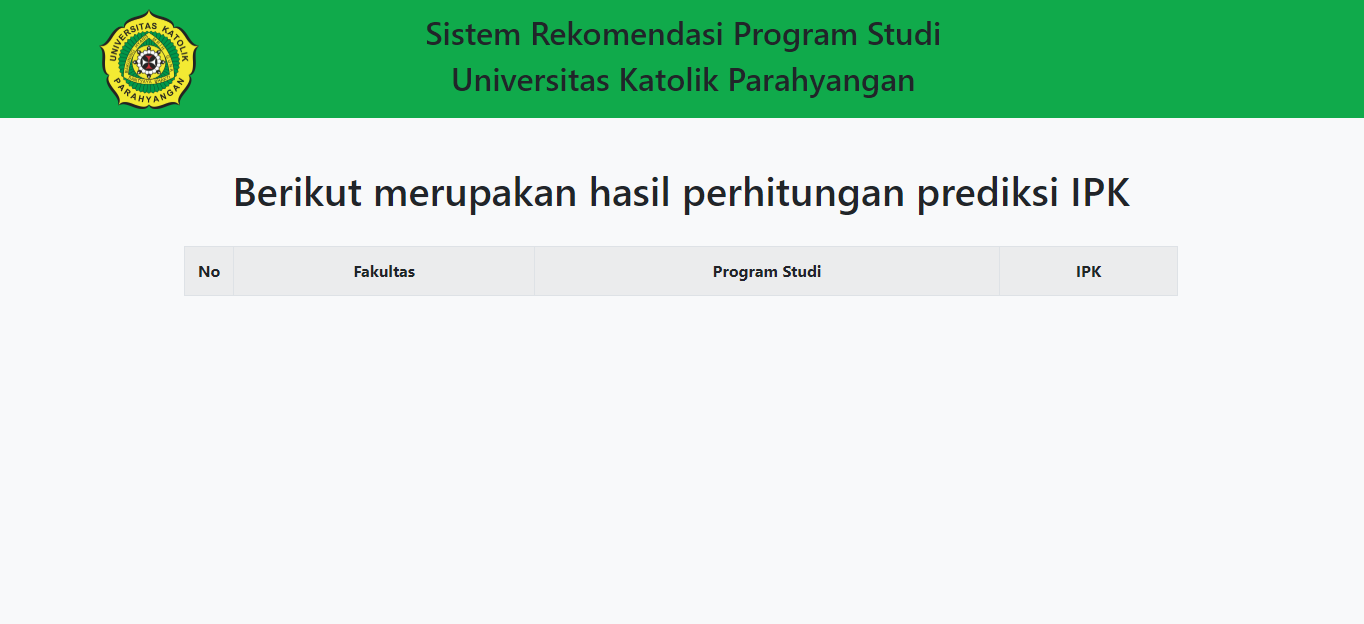
\includegraphics[width = 12cm, height =8 cm]{doc/DokumenSkripsi/Gambar/gambar54.png}
        \caption{Halaman Hasil Rekomendasi}
        \label{fig:gambar54}
    \end{figure}
\end{enumerate}

\section{Pengujian Fungsional}
\label{sec:pengujian fungsional}

Pengujian ini dilakukan untuk menguji fitur-fitur yang ada pada sistem rekomendasi program studi Universitas Katolik Parahyangan agar dapat berjalan dengan baik.

\subsection{Pengujian Fungsional Pemilihan Jurusan SMA}
\label{subsec:pengujian fungsional}

Pengujian ini dilakukan pada fitur pemilihan jurusan saat SMA oleh siswa/i yang menjadi target sistem.

\begin{table}[H]
    \centering
    \begin{tabular}{|c|p{3.5cm}|p{3.5cm}|p{3.5cm}|p{2cm}|}
        \hline
        No & Langkah Pengujian & Hasil yang diharapkan & Hasil Pengujian & Status \\
        \hline
        1 & Memilih juruusan saat SMA & Sistem mengarahkan kepada form sesuai jurusan SMA & Sesuai\\
        \hline
    \end{tabular}
    \caption{Tabel Pengujian Fungsional Pemilihan SMA}
    \label{tab:tabel pengujian fungsional pemilihan SMA}
\end{table}

\subsection{Pengujian Fungsional Pengisian Nilai}
\label{subsec:pengujian fungsional}

Pengujian ini dilakukan pada fitur pengisian nilai mata pelajaran sesuai dengan jurusan saat SMA pada kelas X dan XI. 

\begin{table}[H]
    \centering
    \begin{tabular}{|c|p{3.5cm}|p{3.5cm}|p{3.5cm}|p{2cm}|}
        \hline
        No & Langkah Pengujian & Hasil yang diharapkan & Hasil Pengujian & Status \\
        \hline
        1 & Mengisi nilai sesuai nilai rapor & Memeriksa valid tidaknya data yang dimasukkan dan memeriksa \textit{range} nilai & Sesuai \\
        \hline
        2 & Klik tombol \textit{submit} & Mengerahkan kepada halaman hasil rekomendasi & Sesuai \\
        3 & Mengisi nilai yang tidak valid & Memberikan pesan data tidak valid & Memberikan pesan tidak valid & Sesuai\\
        \hline
    \end{tabular}
    \caption{Tabel Pengujian Fungsional Pengisian Nilai}
    \label{tab:tabel pengujian fungsional pengisian nilai}
\end{table}


\section{Pengujian Eksperimental}
\label{sec:pengujian eksperimental}

Pada subab ini, akan dilakukkan pengujian sistem rekomendasi program studi Universitas Katolik Parahyangan. Pengujian dilakukan menggunakan \textit{Mean Absolute Error} (MAE), \textit{Root Mean Square Error} (RMSE), dan eksekusi waktu program. Data yang digunkan pada pengujian adalah seluruh data mahasiswa yang dibagi menjadi dua yaitu \textit{train set} sebesar 70\% dan \textit{test set} sebesar 40\%.

\subsection{\textit{Mean Absolute Error} (MAE)}
\label{subsec:mae}

\subsection{\textit{Root Mean Square Error} (RMSE)}
\label{subsec:rmse}

\subsection{Eksekusi Waktu Program}
\label{subsec:eksekusi waktu program}